\documentclass[a4paper]{jarticle}
\usepackage{tani_resume}
\usepackage{epstopdf}
\usepackage{graphicx}
\usepackage{ascmac}
\alignbeforeskip -5mm
\alignafterskip -5mm
\eqnarraybeforeskip -5mm
\eqnarrayafterskip -5mm
\makeatletter
\newenvironment{figurehere}
  {\def\@captype{figure}}
  {}
\makeatother

\jptitle{France-IOI提供の国際情報科学コンテストBebras Challenge用コンテスト環境bebras-platformの試運用}
\etitle{}
\jpauthor{鈴木一至 佐々木陽広}
\eauthor{Kazushi Suzuki,Akihiro Sasaki}
\course{谷聖一研究室}
\year{27}


%% 概要 %%
\abstract{
コンピュータ・サイエンスの普及を目的とした取り組みは,様々なところで行われている.
その中の1つに,小・中・高校生を対象にした「Bebras Challenge」がある.Bebras Challengeは,情報科学に触れてもらうことを目的とし,情報科学の事前知識がなくても解くことが可能なオンラインコンテストである.Association France-IOIがBebras Challenge実施用のサーバシステムである「bebras-platform」を開発し,オープンソースとして公開している.bebras-platformには,コンテストを実施するだけでなく,過去に行ったコンテストへ挑戦できる機能もある.本演習では,bebras-platformを利用して,日本でのコンテストサーバ運用のノウハウ蓄積と,過去に実施されたBebras Challengeの問題へ挑戦できる環境を構築した.}
\compheading

\begin{document}
\maketitle
\begin{multicols}{2}
\setcounter{page}{1}

\section{はじめに}

\subsection{Bebras Challenge}
\subsubsection{Bebras Chalengeの概要}
Bebras Challenge (\cite{bebras-contest, bebras-pdf})とは,2004年にリトアニアで始められた国際的な情報科学コンテストである.年に1回実施され,日本では,小学5年生から高等学校3年生を対象としている.日本は2011年度から正式参加しており,2015年には世界35カ国から130万人の児童・生徒が参加している.情報科学の事前知識がなくても解くことが可能な問題を扱い,問題に取り組むことによって情報科学の基礎概念に触れることができ,論理的思考の向上の一助になるようなものになっている.また,コンテスト後に参加者同士で問題の内容について議論することで,情報科学に興味を持つきっかけになることが期待される.

\subsubsection{Bebras Challengeの形式}
 コンテストはオンラインで実施され,参加者はWebブラウザなどを通して参加する.コンテストの問題は年齢に応じた区分ごとに用意されており,基本はベンジャミン(小学5年生・6年生),カデット(中学1年生・2年生),ジュニア(中学3年生・高校1年生),シニア(高校2年生・3年生)の4区分であり,日本ではベンジャミンが30分10問,その他が40分12問で実地している.
\\ 問題形式は大きく2種類あり,動的にオブジェクトを操作しながら試行錯誤できる対話型と,それに対する非対話型がある.また,非対話型の中には選択肢を選んで解く選択肢型と,文字を入力して解答する文字入力型がある.

\subsection{国際情報オリンピック}
国際情報オリンピック(International Olympiad in Informatics, IOI)(\cite{ioi})とは,1989年から毎年行われる中高生を対象としたアルゴリズム設計の能力を競う国際大会である.高校生までの生徒を対象とし,その能力の育成を助け,各国の選手・教育者同士の国際交流を図ることを目的をする.
\\ 日本では,国際情報オリンピックに日本代表選手を派遣するために,情報オリンピック日本委員会が日本情報オリンピックを主催している(詳細は\cite{joi}を参照).
\\ その一部門として,数理情報科学の復旧・啓発のために,主に小中学生向けのイベントの開催やウェブコンテンツの開発・公表を行っている情報オリンピック日本委員会ジュニア部会がある.Bebras Challengeは,このジュニア部会によって実施されている.


\subsection{Association France-IOI}
Association France-IOIは,国際情報オリンピックのフランスチームの選出と育成を目的とし2004年に設立された.フランスでのBebras Challengeを実施しており,Bebras Challenge実施用のサーバシステムであるbebras-platformをオープンソースとして公開している.
\\ Association France-IOIは,2011年からBebras Challengeを実施しており,2015年には世界各国で最も多い35万人もの参加者を集めている.
\subsection{演習目的}
Bebras Challengeを実施するためには,コンテスト環境を提供するサーバシステムが必要であるが,リトアニア,オランダ,フィンランド,台湾,フランスなどの国はサーバシステムを開発し運用している.日本ではオランダのサーバを利用しBebras Challengeを実施しているが,コンテストに参加する教育機関のコンテンツフィルターやファイヤーウォール機器の性能も含めたネットワーク環境によっては,正常にコンテストに参加することが困難な場合があった.
\\ この問題を緩和する方法の1つとして,ネットワーク的に近いコンテストサーバを用意するという方法があげられる.Association France-IOIによるオープンソースのサーバシステムであるbebras-platformを利用し,ネットワーク的に近いコンテストサーバを運用することで,正常にコンテストに参加できない教育機関の減少が期待できる.本演習の目的は,このbebras-platformを用いてBebras Challengeのコンテストサーバを運用するためのノウハウの蓄積と,事後学習のための過去に実施されたコンテストの問題にいつでも挑戦できる練習環境の提供である.

\section{bebras-platform}


\subsection{構成}
bebras-platformは,サーバ全体ではなくHTMLやPHPなどのファイルやデータベースを構成する要素の集合体である.サーバ環境を構築する上では,httpdとして「Apache」,データベースマネージメントシステムとして「MySQL」を利用することが前提とされている.しかしサーバ環境のOSには制約はなく,開発者のニーズに合ったOSを選択することが可能となる.また,bebras-platformはオープンソースソフトウェアであるため,随時変更・改変が行われる.

\subsection{使用ツール}
\begin{description}
\item[Git]プログラムのソースコードなどの変更履歴を記録・追跡するための分散型バージョン管理システムである(\cite{git}).また,Gitを使用してソフトウェア開発プロジェクトのための共有ウェブサービスとしてGitHubがある.\\ bebras-platformは,GitHub上で公開されており,随時更新が行われている.
\end{description}

\begin{description}
\item[Bower]Twitter社によるフロントエンド用パッケージ管理ツールである(\cite{bower}).JSON形式の設定ファイルを用意することで,記述されたパッケージを一括で取り込むことができる.\end{description}

\begin{description}
\item[Composer] PHPの依存関係管理ツールである(\cite{composer}).Bowerと同様にJSONファイルから複数のパッケージのインストールが可能である.
\end{description}

\begin{description}
\item[DBV]  Webページ上でデータベース管理を行うためのツールである(\cite{dbv}).主にAssociation France-IOIのプロジェクトに使用される.\end{description}

\begin{description}
\item[i18next] フロントエンドにて国際化を可能にするライブラリである(\cite{i18n}).JSONと呼ばれるデータ記述形式に対応する訳を記入することで,対応する文字列を翻訳することが可能である.%\\bebras-platformのHTML上では,data-i18n属性を用い,それぞれ翻訳箇所に任意の文字列を入力し使用する.
\end{description}

\subsection{ページ構造}
bebras-platformのユーザ用のページは2種類存在する.1つは,コンテスト参加者が利用するページである(図\ref{fig:1}).コンテストの参加や過去問の参照を行うことができる.
\begin{figurehere}
\begin{center}
\fbox{
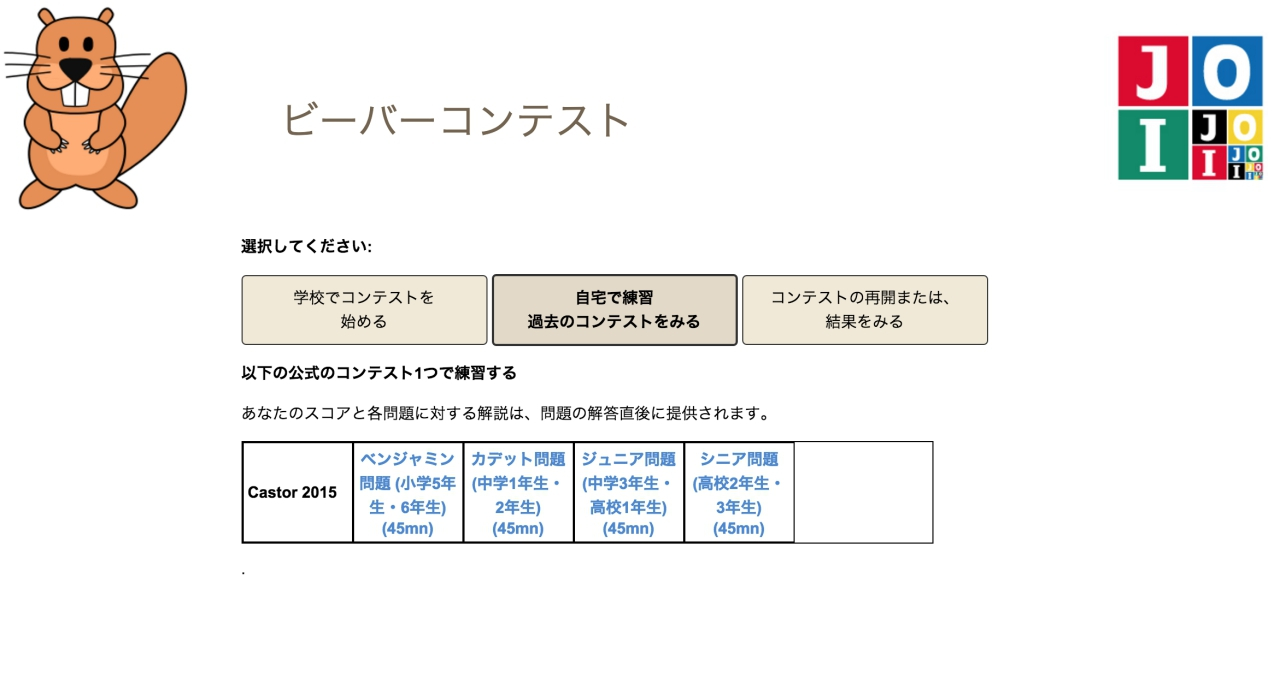
\includegraphics[bb=0 0 1280 679,width=8cm]{img/bebras_top.jpg}
}
\end{center}
\caption{bebras-platformの参加者用ページ}\label{fig:1}
\end{figurehere}

もう1つは,管理者が利用するページである(図\ref{fig:2}参照).コンテストサイトの管理者がログインし,コンテストの作成や問題の追加を行うことができる.

\begin{figurehere}
\begin{center}
\fbox{
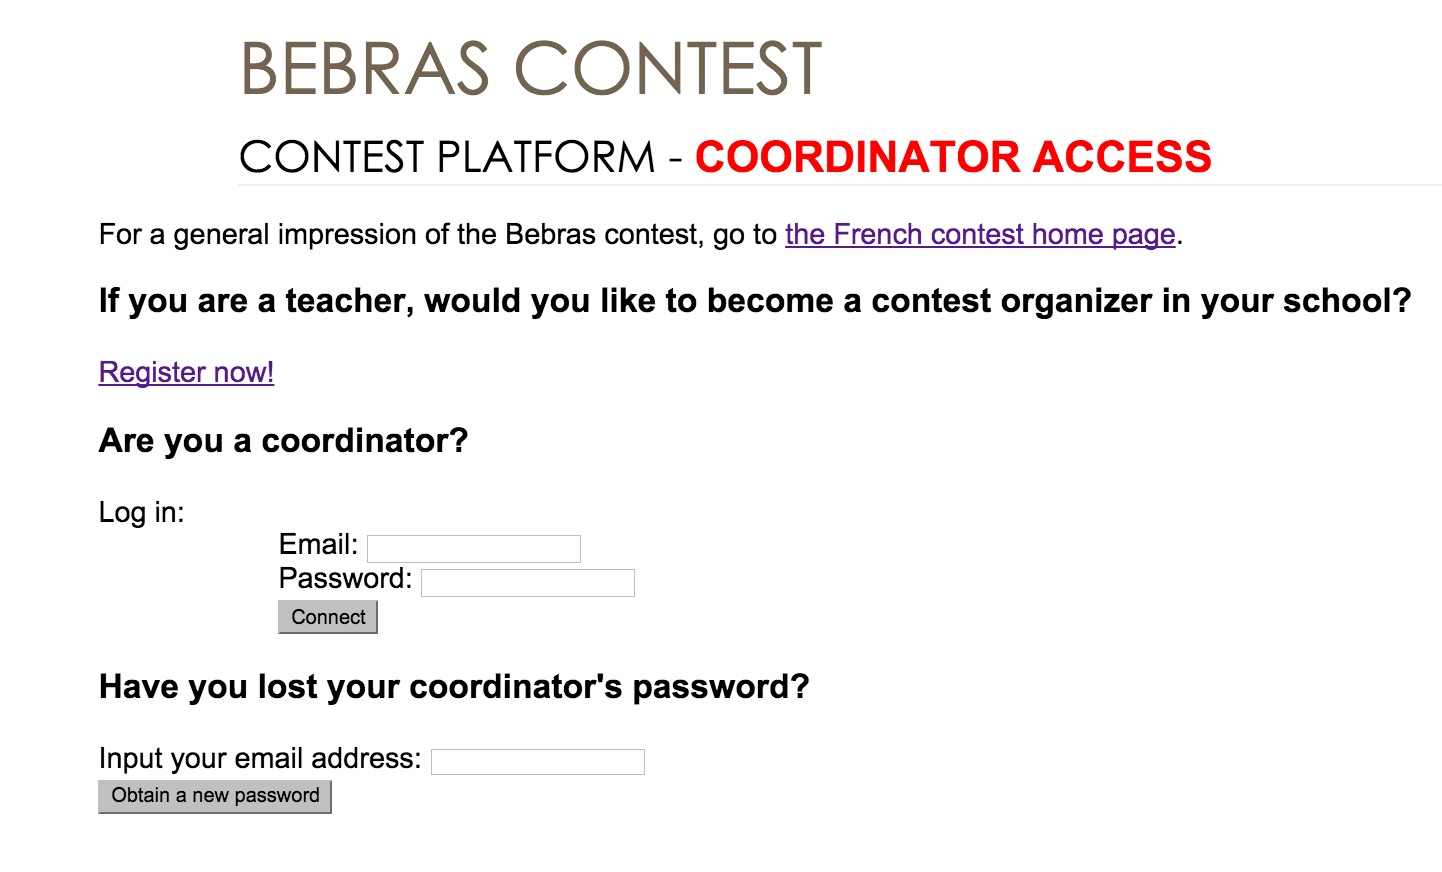
\includegraphics[bb=0 0 1442 872,width=8cm]{img/admin_top.jpg}
}
\end{center}
\caption{bebras-platformの管理者用ページ}\label{fig:2}
\end{figurehere}



\subsection{ユーザ}
\begin{description}
\item[管理者]  ユーザの中で最も強い権限を持ち,問題の追加,コンテストの作成や自分以外のユーザの認証が可能である.ただし最初の管理者の登録はデータベースを直接変更する必要がある. 
\end{description}

\begin{description}
\item[教師] 管理者とは異なる権限を持ち,問題やコンテストの作成はできないが,コンテストの行うためのグループの作成が可能なユーザである.教師はユーザ登録後に管理者に認証してもらう必要がある.
\end{description}

\begin{description}
\item[参加者] 管理者,教師以外のユーザとして参加者がある.参加者は,コンテストの参加,過去問の参照が可能となっており,コンテスト参加時に発行されるアクセスコードを入力することで,コンテストの結果を参照することも可能である.
\end{description}




\section{bebras-platformの試運用}
\subsection{コンテスト環境の構築}
\subsubsection{翻訳}
bebras-platformのインターフェイスは大部分が英語であり,また一部はフランス語で記述されている.コンテスト参加者がスムーズにコンテストを受けるためには,インターフェイスの日本語化が必要不可欠である.そこでi18nextを利用し日本語対応を行った.しかし,日本語化が必要な文字列の中に,i18nextで対応していない形でコード内に埋め込まれている箇所がある.これらについては,直接コードの変更を行い対応した.

\subsubsection{過去問の追加}
2014,2015年度の過去のコンテスト問題を事後学習のための過去問として公開した.問題自体はHTMLファイルで記述されている.非対話型問題については,bebras-platformのサンプル問題を参考にテンプレートHTMLファイルを最初に作成した.以後は,そのテンプレートを編集し,必要に応じて画像などの追加を行い問題ファイルを作成した.問題ファイル作成後は,bebras-platform上で年度や階級ごとにコンテストへ取り込むといった流れになっている.
\\ 対話型問題については,解答方法が一意でないため,非対話型問題のようなテンプレートを作成することができなかった.そのため,
本演習では,対話型問題への対応は今後の課題とし,
%一部機能の実装となっているため,
非対話型の問題形式のみ追加を行った.

\subsection{開発管理環境}
bebras-platformは,随時GitHubにて更新されるため,コンテストサイトを外部へ公開するまでの運用手順を明確化する必要があった.本演習では,一度手元の環境でサーバシステムを構築し,ローカル環境をそのまま本番環境へコピーする形で運用している.このようにすることでBowerなどの管理系ツールを本番環境へ導入する必要がなくなり,更にローカル環境で一度実装することによって本番環境での不具合によるリスクを減らすことが可能である.

\subsection{ドキュメント作成}
bebras-platformはAssociation France-IOI提供のシステムであるため,日本語での記載は一切なく,実装に至るまで様々な試行錯誤を経た.この複雑化したbebras-platformの仕様の明確化と,蓄積したノウハウの共有を目的としたドキュメントの作成を行った.このドキュメントは環境構築手順から現在の運用状況など,報告者以外の人がbebras-platformを手間なく理解するための仕様書である.bebras-platformはAssociation France-IOIによって随時更新されるため,必要に応じてこのドキュメントも整理することが今後重要である.

\section{終わりに}
本演習では,Association France-IOIによるbebras-platformを利用して,Bebras Challenge用コンテスト環境を構築した.
\\ 追加した過去のコンテスト問題は非対話型問題のみの対応となっているため,対話型問題の実装が今後の課題となる.また,過去問を追加するにあたってテンプレートHTMLファイルを作成したが,問題の選択肢,解答などの要素をそれぞれ手動で入力する必要があるため,この問題作成までの一連の流れの自動化が,今後の課題の1つとしてあげられる.
\\ bebras-platformを構築する際に.i18nextに対応していない箇所や細かいバグなどを発見し,修正を行ったが,こういった不具合をFrance-IOIには報告していない.そのため,France-IOIへのフィードバックや,日本語対応したブランチの作成なども今後の課題となる.
\\ bebras-platformを利用し,過去のコンテスト問題に挑戦できる練習環境だけでなく,実際のBebras Challengeの実施も視野入れていたが,bebras-platformの環境構築と時期が合わず,2015年度での実施はできなかった.そのため2016年度以降のBebras Challengeのbebras-platformでの実施や,リトアニアやフィンランドのコンテスト環境の評価も今後の課題である.

\end{multicols}

%%%%% 参考文献 %%%%%
\begin{thebibliography}{1}

\bibitem{bebras-contest} 「ビーバーコンテスト」情報ページ.  http://bebras.eplang.jp/ , (
参照 2016-02-05)
\bibitem{bebras-pdf} 谷 聖一, 兼宗 進, 井戸坂 幸男. 小中高生向け国際情報科学コンテストBebras.  http://www.ipsj.or.jp/magazine/9faeag0000005al5-att/peta55-11.pdf, (参照 2016-02-05)
\bibitem{bebras-france-platform} Bebras Platform. https://github.com/France-ioi/bebras-platform(参照 2016-02-05)
\bibitem{ioi} 国際情報オリンピック http://www.ioinformatics.org/index.shtml   http://www.ioi-jp.org/ioi/(参照 2016-02-05)
\bibitem{joi}日本情報オリンピック委員会 https://www.ioi-jp.org/(参照 2016-02-05)
\bibitem{git} Git  https://ja.wikipedia.org/wiki/Git(参照 2016-02-05)
\bibitem{bower}Bower  http://bower.io/(参照 2016-02-05)
\bibitem{composer}Composer  https://getcomposer.org/(参照 2016-02-05)
\bibitem{dbv}dbv  http://dbv.vizuina.com/(参照 2016-02-05)
\bibitem{i18n}i18n  http://i18next.com/(参照 2016-02-05)



\end{thebibliography}

\end{document} 




